%%%% Paramétrage du TD %%%%
\def\xxactivite{Application 1 \ifprof -- Corrigé \else \fi} % \normalsize \vspace{-.4cm}
\def\xxauteur{\textsl{Xavier Pessoles}}

\def\xxnumchapitre{Chapitre 3 \vspace{.2cm}}
\def\xxchapitre{\hspace{.12cm} Caractéristation inertielle des solides}
%
\def\xxtitreexo{Application -- Vilebrequin de moteur}
\def\xxsourceexo{\hspace{.2cm} \footnotesize{C. Gamelon \& P. Dubois}}
%\def\xxauteur{\textsl{Xavier Pessoles}}


\def\xxcompetences{%
\textsl{%
\textbf{Savoirs et compétences :}\\
\begin{itemize}[label=\ding{112},font=\color{ocre}] 
\item B2-10 : Déterminer les caractéristiques d'un solide ou d'un ensemble de solides indéformables.
\end{itemize}
}}
\def\xxfigures{
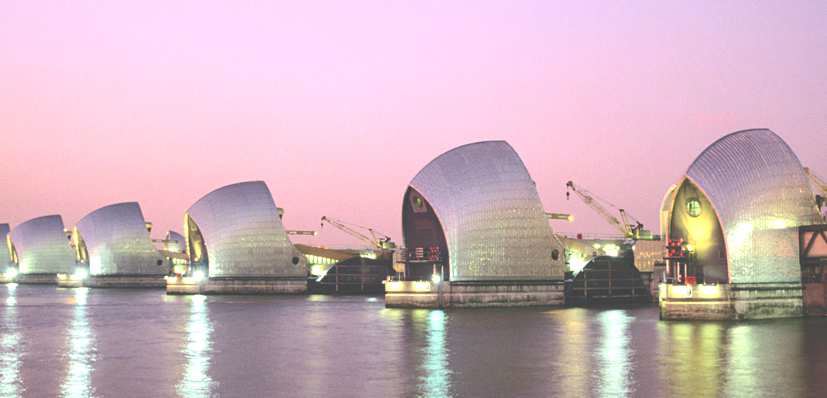
\includegraphics[width=.7\linewidth]{fig_00}
}%figues de la page de garde


\input{\repRel/Style/pagegarde_TD}

\setlength{\columnseprule}{.1pt}

\pagestyle{fancy}
\thispagestyle{plain}

\vspace{5.2cm}

\def\columnseprulecolor{\color{ocre}}
\setlength{\columnseprule}{0.4pt} 

%%%%%%%%%%%%%%%%%%%%%%%

\setcounter{numques}{0}

\ifprof
%\begin{multicols}{2}
\else
\begin{multicols}{2}
\fi


\ifprof
\else
Un vilebrequin est réalisé en mécanosoudage pour faire fonctionner un prototype de moteur. Les géométries sont par conséquent simples : assemblage de tôles ou cylindres en acier.

\begin{center}
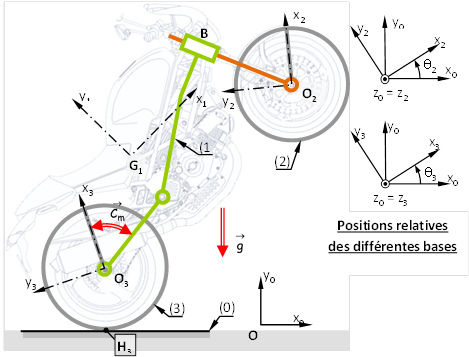
\includegraphics[width=\linewidth]{fig_01}
\end{center}
L'origine $O$ repère $\mathcal{R}$ est située dans le plan de contact du cylindre 1 et du parallélépipède 2.

On note $\rho=\SI{7200}{kg.m^{3}}$ la masse volumique du matériau et on donne :
\begin{multicols}{2}
\begin{itemize}
\item $a = \SI{20}{mm}$;
\item $b = \SI{30}{mm}$;
\item $e = \SI{5}{mm}$;
\item $l = \SI{20}{mm}$;
\item $r = \SI{5}{mm}$;
\item $L = \SI{50}{mm}$;
\item $r_4 = \SI{7.5}{mm}$;
\item $h = \SI{20}{mm}$.
\end{itemize}
\end{multicols}
\fi

\question{Calculer les masses des différentes pièces: $m_1$, $m_2$, $m_3$ et $m_4$.}

\ifprof \begin{corrige}
On a: 
\begin{itemize}
\item $m_1 = \mu \pi r_1^2 l_1$;
\item $m_2 = \mu a b e$
\item $m_3 = \mu \dfrac{1}{2}\pi R^2 e$;
\item $m_4 = \mu \pi r_3^2L$.
\end{itemize}
\end{corrige}
\else
\fi


\question{Déterminer le centre d’inertie de chaque pièce.}
\ifprof \begin{corrige}
On a: 
\begin{itemize}
\item $\vect{OG_1} = h\vect{y}+\dfrac{l_1}{2}\vect{z}$;
\item $\vect{OG_2} = \dfrac{b}{2}\vect{y}-\dfrac{e}{2}\vect{z}$;
\item $\vect{OG_4} = -\left(e+\dfrac{L}{2}\right)\vect{z}$.
\end{itemize}

Le solide 3 a deux plans de symétrie : $\left(\vect{x},\vect{y}\right)$ et $\left(\vect{y},\vect{z}\right)$. On ne cherche donc la composante du centre d'inertie que dans la direction $\vect{y}$.

$m_3 \vect{OG_3}\cdot \vect{y} = \int \vect{OP}\vect{y} \text{d}m$ avec $\text{d}m=\mu \rho \text{d}\rho\text{d}\theta e $ ($\rho$ variant de 0 à $R$ et $\theta$ variant de $-\pi$ à 0) et 

$\vect{OP}=\rho\left( \cos\theta \vect{x}+ \sin\theta \vect{y}\right)$. 

On a donc : 

$ \mu \dfrac{1}{2}\pi R^2 e \vect{OG_3}\cdot \vect{y} = \int \rho\left( \cos\theta \vect{x}+ \sin\theta \vect{y}\right) \vect{y} \mu e\rho \text{d}\rho\text{d}\theta $

$ \Leftrightarrow \dfrac{1}{2}\pi R^2  \vect{OG_3}\cdot \vect{y} = \int \rho^2 \sin\theta  \vect{y} \rho \text{d}\rho\text{d}\theta $
$ \Leftrightarrow \dfrac{1}{2}\pi R^2  \vect{OG_3}\cdot \vect{y} = -\dfrac{R^3}{3}  \left[\cos\theta \right]_{-\pi}^0  \vect{y}$

$ \Leftrightarrow \dfrac{1}{2}\pi  \vect{OG_3}\cdot \vect{y} = -2\dfrac{R}{3}  $
$ \Leftrightarrow  \vect{OG_3}\cdot \vect{y} = -4\dfrac{R}{3\pi}  \vect{y} $

Au final : 
$\vect{OG_3} = -\dfrac{4R}{3\pi}  \vect{y}-\dfrac{e}{2}\vect{z}$
\end{corrige}\else\fi

\question{Déterminer la valeur de $R$ afin que le centre d’inertie du vilebrequin soit sur son axe de rotation. Faire l’application numérique.}

\ifprof \begin{corrige}
On a $\left( m_1+m_2+m_3+m_4\right) \vect{OG}\cdot \vect{y}=0 $

$\Leftrightarrow m_1 \vect{OG_1}\cdot \vect{y}+m_2 \vect{OG_2}\cdot \vect{y}+m_3 \vect{OG_3}\cdot \vect{y}+m_4 \vect{OG_4}\cdot \vect{y} = 0$

$\Leftrightarrow \left(\mu \pi r_1^2 l_1\right) h+\left(\mu a b e\right) \dfrac{b}{2}-\left(\mu \dfrac{1}{2}\pi R^2 e\right) \dfrac{4R}{3\pi} +\left(\mu \pi r_3^2L\right) \cdot 0 = 0$


$\Leftrightarrow  \pi r_1^2 l_1 h+a b e \dfrac{b}{2}- \dfrac{1}{2} R^2 e \dfrac{4R}{3}  = 0$

$\Leftrightarrow  \pi r_1^2 l_1 h\dfrac{3}{2}+a b^2 e \dfrac{3}{4}=  R^3 e  $
$\Leftrightarrow   R^3 = \pi r_1^2 l_1 h\dfrac{3}{2e}+a b^2 \dfrac{3}{4}    $
\end{corrige}\else\fi

\question{Donner les formes des matrices d’inertie de chaque pièce au point où elles s’expriment de manière la plus simple et dans la base $\base{x}{y}{z}$.}
\ifprof \begin{corrige} ~\\

$\inertie{G_1}{S_1}=\matinertie{A_1}{A_1}{C_1}{0}{0}{0}{R}$
$\inertie{G_2}{S_2}=\matinertie{A_2}{B_2}{C_2}{0}{0}{0}{R}$
$\inertie{G_3}{S_3}=\matinertie{A_3}{B_3}{C_3}{0}{0}{0}{R}$
$\inertie{G_4}{S_4}=\matinertie{A_4}{A_4}{C_4}{0}{0}{0}{R}$
\end{corrige}\else\fi

\question{Donner les formes de matrices d’inertie du vilebrequin en $O$ dans la base $\base{x}{y}{z}$.}

\ifprof \begin{corrige}

$\vect{OG_1} = h\vect{y}+\dfrac{l_1}{2}\vect{z}$

$\inertie{O}{S_1}=\matinertie{A_1}{A_1}{C_1}{0}{0}{0}{R}
+m_1\matinertie{h^2+\dfrac{l_1^2}{4}}{\dfrac{l_1^2}{4}}{h^2}{-\dfrac{hl_1}{2}}{0}{0}{R}$

$\vect{OG_2} = \dfrac{b}{2}\vect{y}-\dfrac{e}{2}\vect{z}$

$\inertie{O}{S_2}=\matinertie{A_2}{B_2}{C_2}{0}{0}{0}{R}
+m_2\matinertie{\dfrac{b^2}{4}+\dfrac{e^2}{4}}{\dfrac{e^2}{4}}{\dfrac{b^2}{4}}{-\dfrac{be}{4}}{0}{0}{R}$

$\vect{OG_3} = -\dfrac{4R}{3\pi}  \vect{y}-\dfrac{e}{2}\vect{z}$

$\inertie{O}{S_3}=\matinertie{A_3}{B_3}{C_3}{0}{0}{0}{R}
+m_3\matinertie{\dfrac{16R^2}{9\pi^2}+\dfrac{e^2}{4}}{\dfrac{e^2}{4}}{\dfrac{16R^2}{9\pi^2}}{-\dfrac{4R}{3\pi}\dfrac{e}{2}}{0}{0}{R}$

$\vect{OG_4} = -\left(e+\dfrac{L}{2}\right)\vect{z}$.

$\inertie{O}{S_4}=\matinertie{A_4}{A_4}{C_4}{0}{0}{0}{R}
+m_4\matinertie{\left(e+\dfrac{L}{2}\right)^2}{\left(e+\dfrac{L}{2}\right)^2}{0}{0}{0}{0}{R}$

On a : 

$\inertie{O}{S}=\matinertie{A}{B}{C}{-D}{0}{0}{R}$
\end{corrige}
\else\fi

Le carter moteur peut être basculé pour l’entretien. Cette opération ne doit normalement pas être effectuée lorsque le moteur fonctionne. Afin de calculer les effets dynamiques engendrés par cette manipulation, il est nécessaire de calculer l’inertie en rotation du vilebrequin par rapport à cet axe de rotation.

\question{Calculer l’inertie en rotation par rapport à l’axe $\vect{OA}$.}
\ifprof \begin{corrige}
$\vect{u}=\dfrac{\vect{OA}}{||\vect{OA}||}=\dfrac{L_1\vect{z}+h\vect{y}}{\sqrt{L_1^2+h^2}}$

$J_{\Delta}=\begin{pmatrix} 0 & u_y &  u_z \end{pmatrix} \matinertie{A}{B}{C}{-D}{0}{0}{R}
\begin{pmatrix} 0 \\ u_y \\  u_z \end{pmatrix}$
$=\begin{pmatrix} 0 & u_y &  u_z \end{pmatrix} 
\begin{pmatrix} 0 \\ Bb-Dc \\  -Db +Cc \end{pmatrix}$

$J_{\Delta}= \left( Bb-Dc\right)u_y + \left( -Db +Cc\right)u_z$

\end{corrige}\else\fi


%\section*{Présentation du support du cours du cours}

\ifprof
\else
\end{multicols}
\fi
%
%\newpage
%Question 2 : Position des centres de gravité:
%$\vect{OG_1}=h/2.\vect{y}+\dfrac{l+e}{2}\vect{z}$,  $\vect{OG_2}=b/2\vect{y}$ $\vect{OG_4} =(L+e)/2.\vect{z}$; 
%Avec Guldin : $(4.\pi.R^3)/3=2.\pi.Z_{G_3}.(\pi.R^2)/2$;  $Z_{G_3}=(4.R)/(3.\pi)$. Ainsi 
%$\vect{OG_3}=-(4.R)/(3.\pi).\vect{y}$.
%
%Question 3 : Calcul de R pour que le centre de gravité de l'ensemble soit sur l'axe de rotation.
%
%$m_1 \vect{OG_1}+m_2 \vect{OG_2} +m_3 \vect{OG_3 }+m_4 \vect{OG_4} \vect{z} =0 $
%
%$\rho.(V_1 \vect{OG_1}+V_2 \vect{OG_2}+V_3 \vect{OG_3}+V_4 \vect{OG_4} \vect{z}=0$
%
%$V_1.b_1+V_2.b_2+V_3.b_3+0=0$
%
%$\pi r^2.l.h+a.b^2/2.e-(\pi R^2)/2.(4.R)/3\pi .e=0$
%
%$R=(3/(2.e).( \pi r^2.l.h+a.b^2/2.e))^{1/3}=\SI{28,4}{mm}$


%\end{document}